\documentclass{standalone}
\usepackage[dvipsnames]{xcolor}
\usepackage{tikz-network}

\definecolor{S}{HTML}{0b6884}
\definecolor{E}{HTML}{50b99a}
\definecolor{Ia}{HTML}{ff5e5b}
\definecolor{Is}{HTML}{ffc847}
\definecolor{R}{HTML}{7b678e}
\definecolor{D}{HTML}{bc4b51}

\definecolor{vuln}{HTML}{80475E}


\begin{document}
  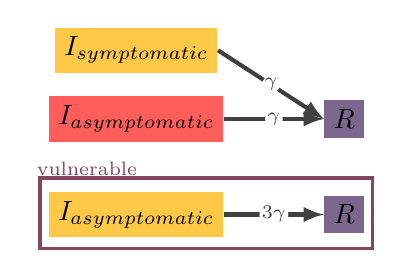
\begin{tikzpicture}[scale=0.66]
    \node at (0,  0.66) (Is) [shape=rectangle, fill=Is] {$I_{symptomatic}$};
    \node at (0, -0.66) (Ia) [shape=rectangle, fill=Ia] {$I_{asymptomatic}$};
    \node at (4, -0.66) (R) [shape=rectangle, fill=R] {$R$};

    \node at (0,  -2.5) (Iav) [shape=rectangle, fill=Is] {$I_{asymptomatic}$};
    \node at (4,  -2.5) (Rv) [shape=rectangle, fill=R] {$R$};

    \draw[very thick, color=vuln] (-1.85,-1.8) rectangle (4.55,-3.15);
    \node at (-2.1,-1.93) [above right, color=vuln]{\scriptsize vulnerable};

    \Edge[Direct, label=$\gamma$](Is.east)(R.west)
    \Edge[Direct, label=$\gamma$](Ia.east)(R.west)
    \Edge[Direct, label=$3\gamma$](Iav.east)(Rv.west)

  \end{tikzpicture}
\end{document}
